% !Mode:: "TeX:UTF-8"
% !TEX program  = xelatex

%\documentclass{cumcmthesis}
\documentclass[withoutpreface,bwprint]{cumcmthesis} %去掉封面与编号页

\usepackage{url}   % 网页链接
\usepackage{subcaption} % 子标题
\title{全国大学生数学建模竞赛编写的 \LaTeX{} 模板}
\tihao{A}
\baominghao{4321}
\schoolname{XX大学}
\membera{}
\memberb{向左}
\memberc{哈哈}
\supervisor{老师}
\yearinput{2017}
\monthinput{08}
\dayinput{22}

\title{微分方程数值解第四周第二次作业}
\begin{document}
	\maketitle
	~\\
	~\\
	
	作业:
	
	$$
	\left\{
	\begin{array}{lcl}
	-(\dfrac{\partial^{2}{u}}{\partial{x^{2}}}+\dfrac{\partial^{2}{u}}{\partial{y^{2}}})=(\pi^{2}-1)e^{x}sin(\pi y) &,&0 \leq x \leq 2,0 \leq y \leq 1 \\
	
	u(0,y)=sin(\pi y),u(2,y)=e^{2}sin(\pi y) &, & 0 \leq y \leq 1 \\
	
	u(x,0)=0,u(x,1)=0,&, &0 \leq x \leq 2
	\end{array}
	\right.
	$$
	
	该问题的精确解为$ u(x,y)=e^{x}sin(\pi y)$.
	
	定义误差为$$ E(h_{1},h_{2})=\max \limits_{1 \leq i \leq M-1 \atop 1 \leq j \leq N-1 } |u(x_{i},y_{j})-u_{ij})| $$
	
	请分析误差在不同步长下的变化情况,验证误差阶,并画出误差图。

	
	
	解:将xM等分,将yN等分。
	
	九点差分格式为
	
	$$-\dfrac{1}{h_{2}^{2}}u_{i,j-1}-\dfrac{1}{h_{1}^{2}}u_{i-1,j}+2(\dfrac{1}{h_{1}^{2}}+\dfrac{1}{h_{2}^{2}})u_{i,j}-\dfrac{1}{h_{1}^{2}}u_{i+1,j}-\dfrac{1}{h_{2}^{2}}u_{i,j+1}=f_{i,j}$$
	
	其中,$ 1 \leq i \leq N-1 ,1 \leq j \leq N-1 $.
	$f_{i,j}=(\pi^{2}-1)e^{x_{i}}sin(\pi y_{j})$.
	

	可用高斯-塞德尔迭代解方程组,迭代式写为
	$$
	u_{i,j}^{k+1}=[f(x_{i},y_{j})+\dfrac{1}{h_{2}^{2}}u_{i,j-1}^{k+1}+\dfrac{1}{h_{1}^{2}}u_{i-1,j}^{k+1}+\dfrac{1}{h_{1}^{2}}u_{i+1,j}^{k}+\dfrac{1}{h_{2}^{2}}u_{i,j+1}^{k}]/[2(\dfrac{1}{h_{1}^{2}}+\dfrac{1}{h_{2}^{2}})]
	$$
	
	$k$表示第k次迭代
	
	~\\
	~\\
	
	
	\textbf{解题程序运行于Matlab 2018a.}
	
	当M=40,N=10时的数值解和精确解对比见图\ref{fig:f5},从图像上看很接近。
	\begin{figure}
		\centering
		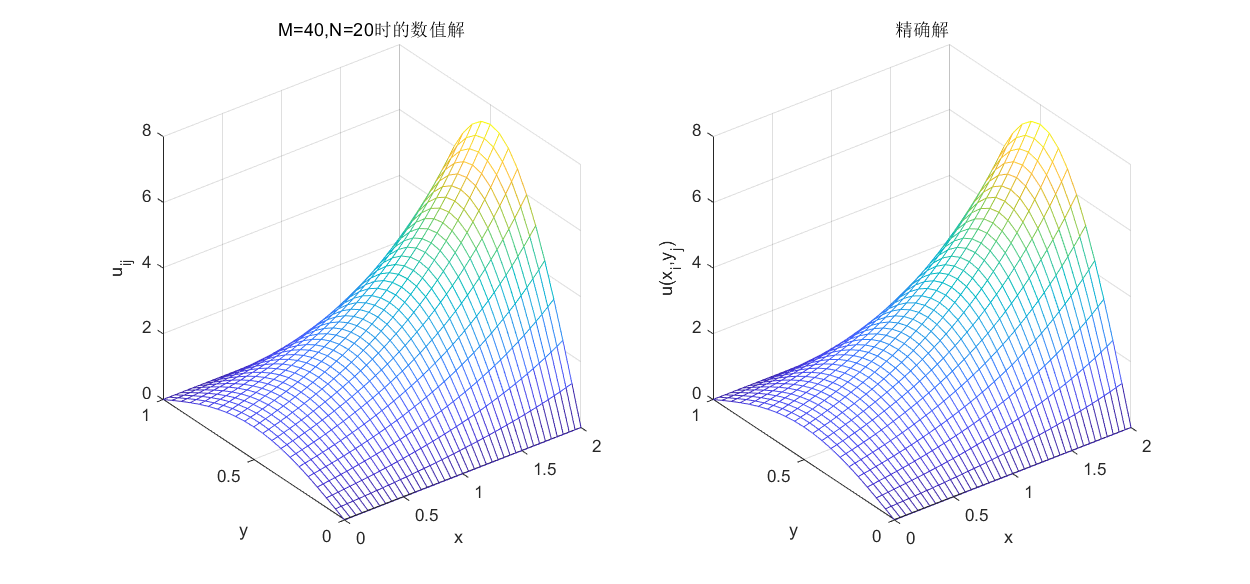
\includegraphics[width=1\linewidth]{figures/f5}
		\caption[M=40,N=20的数值解和精确解]{}
		\label{fig:f5}
	\end{figure}
	
	当取不同的M和N时,数值解在一些点上的取值和精确解见表\ref{tab:1},可知,当区间数越大,即步长越小,数值解越接近与精确解。
	% Table generated by Excel2LaTeX from sheet 'Sheet1'
	\begin{table}[htbp]
		\centering
		\caption{不同的M和N时,数值解在一些点上的取值和精确解}
		\begin{tabular}{crrrr}
			\multirow{2}[0]{*}{M,N} & \multicolumn{4}{c}{x(y=0.5)} \\
			& \multicolumn{1}{c}{0.4} & \multicolumn{1}{c}{0.8} & \multicolumn{1}{c}{1.2} & \multicolumn{1}{c}{1.6} \\
			20,10 & 1.4918055414  & 2.2255083825  & 3.3200724539  & 4.9529855650  \\
			40,20 & 1.4918235062  & 2.2255389042  & 3.3201141569  & 4.9530295099  \\
			80,40 & 1.4918246233  & 2.2255408021  & 3.3201167501  & 4.9530322425  \\
			160,80 & 1.4918246930  & 2.2255409206  & 3.3201169119  & 4.9530324130  \\
			精确解   & 1.4918246976  & 2.2255409285  & 3.3201169227  & 4.9530324244  \\
		\end{tabular}%
		\label{tab:addlabel}%
	\end{table}%
	
	
	
	取不同M和N时,误差见图\ref{fig:2},M和N越大,误差越小。
	
	 \begin{figure*}
		\centering
		\begin{subfigure}[b]{0.475\textwidth}
			\centering
			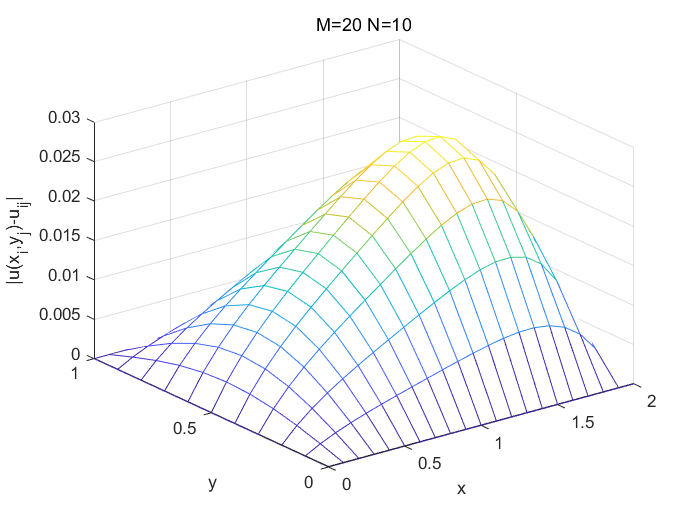
\includegraphics[width=\textwidth]{figures/f1}
			\caption[Network2]%
			{{\small M=20,N=10时的误差}}    
			\label{fig:mean and std of net14}
		\end{subfigure}
		\hfill
		\begin{subfigure}[b]{0.475\textwidth}  
			\centering 
			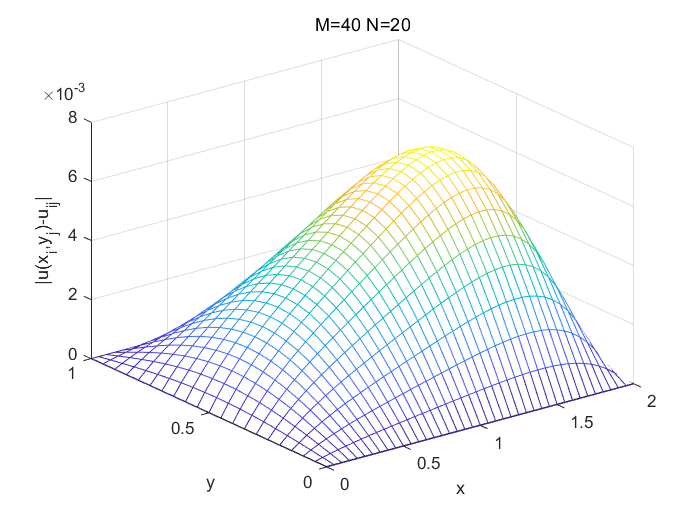
\includegraphics[width=\textwidth]{figures/f2}
			\caption[]%
			{{\small M=40,N=20时的误差}}    
			\label{fig:mean and std of net24}
		\end{subfigure}
		\vskip\baselineskip
		\begin{subfigure}[b]{0.475\textwidth}   
			\centering 
			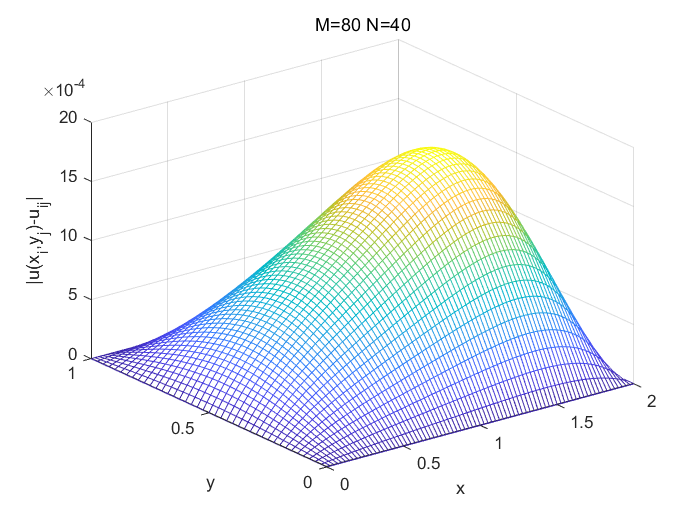
\includegraphics[width=\textwidth]{figures/f3}
			\caption[]%
			{{\small M=80,N=40时的误差}}    
			\label{fig:mean and std of net34}
		\end{subfigure}
		\quad
		\begin{subfigure}[b]{0.475\textwidth}   
			\centering 
			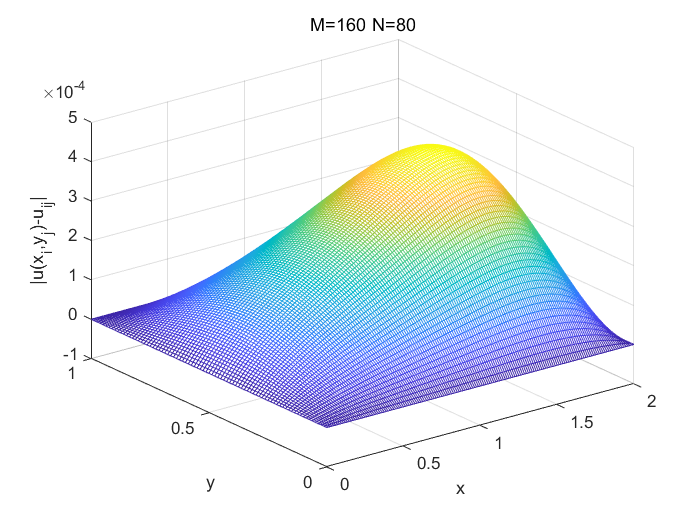
\includegraphics[width=\textwidth]{figures/f4}
			\caption[]%
			{{\small M=160,N=80时的误差}}    
			\label{fig:mean and std of net44}
		\end{subfigure}
		\caption[ The average and standard deviation of critical parameters ]
		{ 取不同M,N的误差} 
		\label{fig:2}
	\end{figure*}


	定义误差阶为
	$$rate=log_{2}(E(2h_{1},2h_{2})/E(h_{1},h_{2}))$$
	求出上述不同M,N对应的步长误差阶,见表\ref{tab:2},误差达到了4阶,为九点差分格式截断误差的阶数。
	% Table generated by Excel2LaTeX from sheet 'Sheet1'
	\begin{table}[htbp]
		\centering
		\caption{不同步长时的误差和误差阶}
		\begin{tabular}{crr}
			\multirow{2}[0]{*}{h1,h2} & \multicolumn{1}{c}{\multirow{2}[0]{*}{E(h1,h2)}} & \multicolumn{1}{c}{\multirow{2}[0]{*}{rate}} \\
			&       &  \\
			1/10,1/10 & 4.84E-05 & \multicolumn{1}{c}{*} \\
			1/20,1/20 & 3.01E-06 & 4.005469 \\
			1/40,1/40 & 1.88E-07 & 4.000988 \\
			1/80,1/80 & 1.18E-08 & 3.999005 \\
		\end{tabular}%
		\label{tab:addlabel}%
	\end{table}%
	
	
\end{document}